\chapter{Multiple sequence alignment}

Sequence alignment, in general, is a task whose purpose is to arrange two or more sequences with a common alphabet to identify similar
and different regions within them. A set of sequences being \emph{aligned} in this case can be understood as each being extended by spaces
in such a way that if they are arranged in a matrix, each sequence occupying one row and each column containing one character, it can be seen
what had to happen for one sequence to change into another on a character-by-character basis: insertion (or deletion), character substitution,
or nothing if the characters in the given position are identical. A good sequence alignment algorithm is one that does not perform
unnecessary insertions (deletions) or substitutions.

The problem of multiple sequence alignment is most studied in bioinformatics. Since DNA was first sequenced
in the 1970s, there has been a need to compare various genomes to determine similarity. As organisms mutate and evolve, their
DNA or RNA changes. Aligning their genomes reveals similar and different regions, which facilitates the tracking of these
mutations and makes it possible to determine the order in which they happened.

However, the applications of sequence alignment are not limited to biology. Every task that makes use of determinig the similarity
of some sequences, where the emphasis is put on finding regions where they do not diverge, can make use of the existing methods.

Melody alignment of Gregorian chant can be considered as such. As the tradition spread across Europe, each place changed some of 
the existing melodies by a little, thereby creating new melodies that can change further as they travel through time and space.
This is akin to the mutations in DNA caused by environmental factors. Finding well-conserved regions in many instances of chant
provides great insight into which parts of a melody are unlikely to change, and, on the other hand, which ones tend to vary
a lot. It can also reveal the ancestors of a melody and the path which it traveled to transform into its final form.
This is in line with the focus of philology shifting not to merely reconstructing an earliest layer of a text (with the unspoken 
assumption that this is the ``real'' text), but to map the entire tradition of text transmission and evolution, taking the later layers 
to be as valid within their cultural environment as the older layers.


In this chapter, we will first give the definition of the problem of sequence alignment. We will mention some important considerations,
as well as theoretical limitations. Then we will provide an overview of the methods developed for bioinformatics that attempt to solve
the problem. Finally, we will show how we applied the existing methods and technologies on Gregorian chant melodies.

\section{The problem of sequence alignment}

Assume that we have an alphabet $\mathcal{A}$ and a character $\sigma$ such that $\sigma \notin \mathcal{A}$. Then let us have a set
of sequences $S = \{s_1, s_2, ..., s_k\}$ with $s_i \in \mathcal{A}^{l_i}$. The output of a sequence alignment algorithm is the set of
aligned sequences $A = \{a_1, a_2, ..., a_k\}$, where $a_k \in (\mathcal{A}\cup\{\sigma\})^L$, $L \geq l_i \:\forall i\in\{1, 2, ..., k\}$.
Each original sequence $s_i$ can be obtained from the aligned sequence $a_i$ by removing all $\sigma$.

Given two aligned sequences $a_i$ and $a_j$ and an index $p \leq L$, we define the following operations:

\begin{itemize}
    \item \emph{Identity}: $(a_i)_k = (a_j)_k$
    \item \emph{Insertion}: $(a_i)_k = \sigma \land (a_j)_k \in \mathcal{A}$
    \item \emph{Deletion}: $(a_i)_k \in \mathcal{A} \land (a_j)_k = \sigma$
    \item \emph{Substitution}: $(a_i)_k \in \mathcal{A} \land (a_j)_k \in \mathcal{A} \land (a_i)_k \neq (a_j)_k$
\end{itemize}

Each of the operations has an associated cost. The cost of substitution can further vary depending on which characters are being
substituted. We can then define the overall cost of the alignment $A$ in different ways, e.g. as the sum of costs over all triples
$(i, j, p) \: \forall i, j \in \{1, 2, ..., k\} \: \forall p \leq L$ or as the sum of costs for unordered pairs $\{i, j\}$ and indices $p$,
in which case insertion and deletion are considered the same operation. The goal of a sequence alignment algorithm is to minimize the cost.
There are other, more complicated ways of defining the cost  function, and the performance of an algorithm is highly dependent on which one it uses.

\subsection{Pairwise and multiple sequence alignment}

Depending on the number of sequences to align, we distinguish between pairwise alignment for pairs of sequences and multiple sequence alignment
for more than two. Despite the similarity in their outcomes, the two problems are fundamentally different from a computational perspective.

Pairwise alignment is relatively easy to solve. The Needleman-Wunsch algorithm, which is a dynamic programming algorithm, can find an optimal
solution in the asymptotic time of $\mathcal{O}(mn)$, where $m$ and $n$ are the respective lengths of the sequences. This means that it is
possible to find an optimal alignment even for longer sequences.

Needleman-Wunsch algorithm can be extended to more than two sequences. However, with each additional sequence, its complexity increases,
and it quickly becomes impractical or even practically impossible to align multiple sequences this way. In fact, it has been proven that multiple sequence
alignment is an NP-complete problem \citep{msa_complexity}. It is therefore necessary to use various heuristics to generate alignments. Current
algorithms do not aim at finding the optimal alignment; instead, they try to produce one that is good enough.

\subsection{Local and global sequence alignment}

There is a distinction to be made between local and global sequence alignment.

The problem description above is the definition of global alignment. Aligning sequences globally means aligning the entire sequences end-to-end.
(This does not mean, however, that there cannot be gaps at the beginning or at the end of the generated alignment.)
All characters from all sequences must be present in the final alignment. Global alignment is used to compare relatively similar
sequences, such as protein homologues or versions of the same chant sung at different points in time.

On the other hand, the goal of local alignment is to find similar regions in divergent sequences, while the rest of the sequences is disregarded.
The output of local alignment algorithms contains only a substring of both sequences. Local alignment is suitable for finding conserved patterns.

Both methods are useful in their own way. Local alignment provides a slightly different insight than global alignment, however, they can
be combined to extract more information. In fact, the best current multiple sequence alignment algorithms use local alignment for pairs
of sequences to generate a better overall global alignment. \citep{msa_overview}

\section{Sequence alignment methods}

The methods used to find sequence alignments depend on how many sequences there are and whether they should be aligned globally or locally.
Dynamic programming can used for finding pairwise alignment, both local and global. For many sequences, other methods have been developed. They
do not compute the optimal alignment, however, by using appropriate heuristics, their output is good enough.

\subsection{Pairwise alignment: dynamic programming}

Dynamic programming techniques are useful for pairwise alignment. The Needleman-Wunsch algorithm \citep{needleman} computes the global alignment
of two sequences. A variation of the algorithm, the Smith-Waterman algorithm \citep{smith_waterman}, computes the local alignment of two sequences.

\subsubsection{Needleman-Wunsch algorithm}

The idea of the algorithm is to start with two empty sequences and subsequently add characters from either or both of the given sequences so as
to obtain an optimal alignment in each step. Namely, suppose that we have two sequence prefixes $A$ and $B$ that have already been aligned optimally
and their alignment gives a score of $s$. Furthermore, suppose that the next characters in the sequences are $a$ and $b$, respectively. There are
three possibilities:

\begin{itemize}
    \item We append $a$ and $b$ to the respective prefixes. By doing so, we obtain the aligned sequence prefixes $Aa$ and $Bb$.
        \begin{verbatim}
            Aa
            Bb
        \end{verbatim}
    \item We append $a$ to $A$ and a gap to $B$. This way, we get the aligned prefixes $Aa$ and $B$.
        \begin{verbatim}
            Aa
            B-
        \end{verbatim}
    \item We append a gap to $A$ and $b$ to $B$. Now we have aligned the prefixes $A$ and $Bb$.
        \begin{verbatim}
            A-
            Bb
        \end{verbatim}
\end{itemize}

Each of the possibilities adds a value to the score $s$ depending on what characters were added. To get the optimal alignment, we choose the one
that yields the highest score. We then proceed to the next character, having two optimally aligned prefixes $A'$ and $B'$. This leads to a recursive
algorithm that can be formulated using dynamic programming.

Let us have two input sequences, $A$ and $B$ of lengths $m$ and $n$ with a common alphabet $\mathcal{A}$ and the gap character $\sigma$.
Let us define the scoring function $s$ as

\[ s(a, b) = 
    \begin{cases}
        1  & \text{if } a = b \\
        -1 & \text{if } a = \sigma \lor b = \sigma \\
        -1 & \text{if }  a \neq b
    \end{cases}
\]

The algorithm initializes a matrix $M$ of size $(m+1) * (n+1)$. The rows and columns represent the characters of $A$ and $B$, respectively, except
for the first row and the first column, which represent the beginning of a sequence or an empty sequence. That is to say, the row $M_{i, *}$ represents the
character $A_{i-1}$ for $i \geq 2$ and analogically, the column $M_{*, j}$ represents the character $B_{j-1}$ for $j \geq 2$.

The algorithm iterates over the rows and columns of the matrix. In each step, it calculates the value of a cell $M_{i,j}$, provided that each of the cells $M_{i-1, j}$,
$M_{i, j-1}$ and $M_{i-1, j-1}$ have been filled out, as

\[ M_{i, j} = max
    \begin{cases}
        M_{i-1, j-1} + s(A_{i-1}, B_{j-1}) \\
        M_{i-1, j} + s(A_{i-1}, \sigma)    \\
        M_{i, j-1} + s(\sigma, B_{j-1})
    \end{cases}
\]

In other words, the algorithm either aligns the two characters in positions $i-1$ and $j-1$, or it inserts a gap into sequence $B$, or it inserts a gap into sequence $A$,
and chooses the version which yields the highest score.

The first row and column are apparently special cases, as there is no previous row or column. Therefore, for each cell in the first row or column, there is
only one possible choice of score, which is equivalent to inserting a space.

After filling out the entire matrix, the algorithm then finds the optimal alignment by backtracking in the matrix. It starts in the bottom right
cell of the matrix, which represents both sequences being aligned. In each iteration, it looks at the cells above, to the left and to the top-left
of the current positions and chooses the highest score. If it moves top or left, it means that a gap was inserted. Moving diagonally represents a match
or mismatch. By tracing its way back to the top left corner, the algorithm finds the alignment that yielded the highest score.

Let us show the algorithm on an example. Consider two sequences of nucleotide residues:

\begin{verbatim}
    GATTA
    GCATG
\end{verbatim}

The matrix is initialized without anything filled out.

% create a figure

\begin{verbatim}
          G  C  A  T  G
      
    G 
    A 
    T 
    T 
    A 
\end{verbatim}

We start filling out the matrix in the top left corner. Using the basic scoring scheme (+1 for a match, -1 for everything else), we insert a 0
to the beginning, and, since there is no top cell for the first row and no left cell for the first column, we add -1 to each subsequent cell,
representing a gap insertion.

\begin{verbatim}
          G  C  A  T  G
       0 -1 -2 -3 -4 -5
    G -1
    A -2
    T -3
    T -4
    A -5
\end{verbatim}

The next cell to fill out is the one in the first \verb|G| column and the first \verb|G| row. We have three options:

\begin{itemize}
    \item Move from the top, represents gap insertion for a score of -1. The final score would be $(-1) + (-1) = -2$.
    \item Move diagonally, represents match, giving a score of +1. The score in this case would be $0 + 1 = 1$.
    \item Move from the left, i.e. gap insertion. The score would be $-2$ as in the first case.
\end{itemize}

We choose the highest score, which in this case is a diagonal move representing a match. It follows intuition: we are now aligning
\verb|G| and \verb|G|, matching them seems logical.

\begin{verbatim}
          G  C  A  T  G
       0 -1 -2 -3 -4 -5
    G -1  1
    A -2
    T -3
    T -4
    A -5
\end{verbatim}

Now let us look at the cell in the \verb|C| column and the \verb|G| row. Moving from the top yields -3, moving from the left yields
0 and moving diagonally yields -2, as it is a mismatch in this case. The highest of these scores is 0.

\begin{verbatim}
          G  C  A  T  G
       0 -1 -2 -3 -4 -5
    G -1  1  0
    A -2
    T -3
    T -4
    A -5
\end{verbatim}

We continue filling out the table this way until it is complete.

\begin{verbatim}
          G  C  A  T  G
       0 -1 -2 -3 -4 -5
    G -1  1  0 -1 -2 -3
    A -2  0  0  1  0 -1
    T -3 -1 -1  0  2  1
    T -4 -2 -2 -1  1  1
    A -5 -3 -3 -1  0  0
\end{verbatim}

As we have now calculated the scores for all prefixes, we can use backtracking to find the optimal alignment for the two sequences.
Starting in the bottom right cell, we choose the cell (top, left or top-left) with the highest score. If multiple cells have the same score, we can 
choose either. The different alignments the cells represent are all optimal. The cell that we choose gives us the optimal alignment
of the sequences before the last character was added. Depending on the direction by which we moved, we know whether this last character
was a character of the sequence or a gap.

For example, consider the bottom right corner of the matrix.

\begin{verbatim}
       T  G
    T  1  1
    A  0  0
\end{verbatim}

Starting in the bottom right, we can choose either the top or the top-left cell. Choosing the top-left one, i.e. moving diagonally, means that
the last characters in the alignment were \verb|A| and \verb|G| for the respective sequences. We can find the alignment of the prefixes \verb|GATT|
and \verb|GCAT| by backtracking from the top-left cell. By contrast, choosing the top cell means inserting a gap in the second sequence, and by backtracking
from there we can find the alignment of \verb|GATT| and \verb|GCATG|.

\begin{figure}[h]
    \begin{equation*}
        \begin{matrix}
                &            & G          & C          & A          & T          & G        \\
                & \rn{00}{0} & -1         & -2         & -3         & -4         & -5       \\
            G   & -1         & \rn{11}{1} & 0          & -1         & -2         & -3       \\
            A   & -2         & 0          & \rn{22}{0} & \rn{23}{1} & 0          & -1       \\
            T   & -3         & -1         & -1         & 0          & \rn{34}{2} & 1        \\
            T   & -4         & -2         & -2         & -1         & \rn{44}{1} & 1        \\
            A   & -5         & -3         & 3          & -1         & 0          & \rn{55}{0}
        \end{matrix}
    \end{equation*}

    \begin{tikzpicture}[overlay,remember picture]
        \draw [->] (55) -- (44);
        \draw [->] (44) -- (34);
        \draw [->] (34) -- (23);
        \draw [->] (23) -- (22);
        \draw [->] (22) -- (11);
        \draw [->] (11) -- (00);
    \end{tikzpicture}
\caption{A path representing an optimal alignment.}
\label{alignment_path}
\end{figure}


Figure \ref{alignment_path} shows a path that represents the alignment

\begin{verbatim}
    G A - T T A
    G C A T - G
\end{verbatim}

\subsubsection{Smith-Waterman algorithm}

The algorithm is similar to Needleman-Wunsch algorithm. As its purpose is to find an optimal local alignment, it does not
penalize long regions of mismatches or gaps. Its purpose is to find regions with the most matches. The only difference from the Needle\-man-Wunsch 
algorithm is in how new matrix cells are filled out. Namely, when willing out a new cell, we use the formula

\[ M_{i, j} = max
    \begin{cases}
        0   \\
        M_{i-1, j-1} + s(A_{i-1}, B_{j-1}) \\
        M_{i-1, j} + s(A_{i-1}, \sigma)    \\
        M_{i, j-1} + s(\sigma, B_{j-1})
    \end{cases}
\]

In other words, all negative values in what would be the matrix from Needle\-man-Wunsch algorithm are replaced by 0.

\subsection{Multiple sequence alignment: progressive methods}

As has already been mentioned, it is essentially impossible to use dynamic programming to compute the alignment of more than two sequences.
Therefore, other methods have been developed. The most successful ones appear to be the so-called progressive methods. In general,
they use some heuristics to estimate a guide tree, which is a phylogenetic tree determining how close the sequences are to each other,
and then they compute the actual multiple alignment following the order of this tree.

One of such methods is the Tree-based Consistency Objective Function for alignment Evaluation (T-Coffee) algorithm \citep{t_coffee}.
Its most important contribution is its extended library generated from both local and global pairwise alignments of all pairs of input sequences.
This library enables the algorithm to make fewer mistakes in the initial stages of the guide tree, as these errors propagate throughout the entire tree.

\begin{figure}[h]
\centering
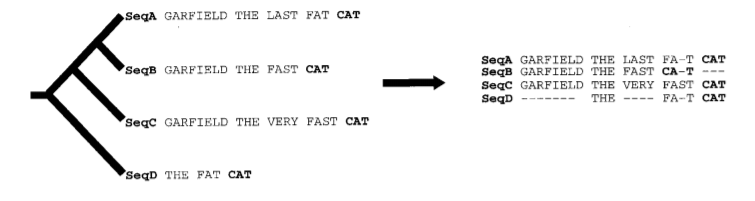
\includegraphics[scale=0.85]{t-coffee-errors}
\caption{Misalignment of the word CAT using other progressive methods. \citep[Figure~2(a)]{t_coffee}}
\end{figure}

Another method is MAFFT (the name presumably coming from the acronyms for multiple alignment and fast Fourier transform) \citep{mafft}.
The authors focused on finding alignments that are not only optimal, but also biologically correct. They developed a way of rapid identification
of homologous regions between two sequences using FFT, and then used the better pairwise alignments to create a better multiple alignment.

\subsubsection{T-Coffee}

The T-Coffee algorithm consists of various stages. The first one is to compute pairwise alignments for all pairs of input sequences.
Two primary libraries are generated, one for global and one for local alignments. Each can contain more than one alignment for each pair.

As some alignments tend to be more correct than others, weighting is then performed. The authors chose sequence identity of two aligned
sequences as the weight of each of the aligned residues in the pair. For example, consider the sequences $A$ \verb|GARFIELD THE LAST FAT CAT|
and $B$ \verb|GARFIELD THE FAST CAT|. If they are aligned as

\begin{verbatim}
    GARFIELD THE LAST FAT CAT
    GARFIELD THE FAST CAT ---
\end{verbatim}

then their sequence identity is 88\%, as there are two non-equal characters aligned (i.e. there is no gap penalty). Therefore, the weight of
each residue pair $W(A(x), B(y))$, where $A(x)$ denotes the character $x$ from sequence $A$, and analogically for $B(y)$, is equal to 88.

\begin{figure}[h]
\centering
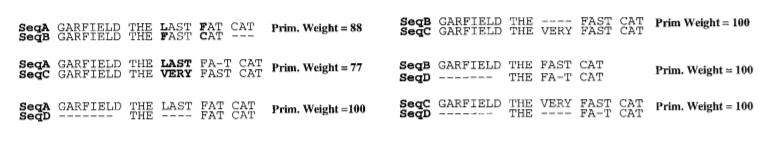
\includegraphics[scale=0.85]{t-coffee-primary-lib}
\caption{Primary library created from 4 sequences. \citep[Figure~2(b)]{t_coffee}}
\end{figure}

The two primary libraries are then combined into one by combining all identical residue pairs into one entry and summing their weights, while
pairs that are only present once are added with their original weight. Residue pairs that are not present in any alignment have an implicit weight
of 0.

Although the information present in the primary library is sufficient to obtain a multiple alignment, it is computationally hard to do so. Instead,
the authors chose to generate what they call an extended library using the weights in the primary library.

Library extension is performed by comparing each aligned residue pair with all the others. Consider a residue pair $(A(x), B(y))$ and a sequence $C$.
The initial weight of the pair is then increased by $min(W(A(x), C(z)), W(C(z), B(y)))$, i.e. the minimum weight associated to the alignment of some
residue $C(z)$ with both $A(x)$ and $B(y)$. This is done for all residues from all sequences. In practice, most of the weights will be 0, therefore 
the actual algorithm computes the weights more efficiently. Library extension in effect computes how consistent a residue-pair alignment is.

\begin{figure}[h]
\centering
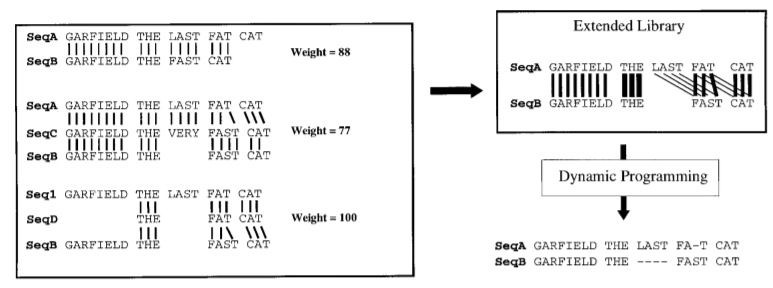
\includegraphics[scale=0.85]{t-coffee-extended-lib}
\caption{Extended library weights for two sequences and their alignment recomputed using these weights. \citep[Figure~2(c)]{t_coffee}}
\end{figure}

Having obtained the consistency information from the extended library, it is now possible to create the guide tree and the final multiple alignment.
Using a distance matrix between all the sequences, the tree is computed as follows. First, we align the closest two sequences using dynamic programming
and the weights from the extended library. In each of the following steps, we either add a sequence to an already computed alignment, or we align
the next closest sequences. We repeat this step until the alignment of all sequences is complete.

\begin{figure}[h]
\centering
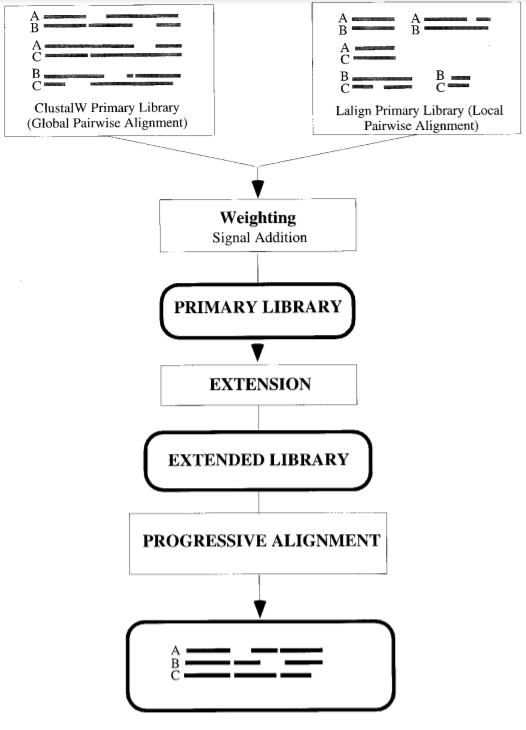
\includegraphics[scale=0.5]{t-coffee-flowchart}
\caption{T-Coffee layout. \citep[Figure~1]{t_coffee}}
\end{figure}

\subsubsection{MAFFT}

The MAFFT method is similar to T-Coffee in that it constructs a library of alignments which it then uses to create the final multiple alignment. The authors developed MAFFT
to work in multiple modes, one of which is the progressive method as described above; the other one is the iterative refinement method, which allows for alterations
of the multiple alignment obtained from the progressive method.

Pairwise alignment in MAFFT uses the fact that certain amino acids have more similar physico-chemical properties than others. Substitutions tend to preserve the
overall structrure of a protein, therefore substitutions of similar amino acids are more frequent than those of different ones. The two properties
the authors use are amino acid volume and polarity.

Let us define the correlation of the volume component between two amino acid sequences with the positional lag of $k$ as

\[
    c_v(k) = \sum_{1\leq n \leq N, 1 \leq n+k \leq M} \hat{v}_1(n) \hat{v}_2(n+k)
\]
where $N$ and $M$ are the lengths of the sequences and $\hat{v}(a) = [v(a) - \bar{v}] / \sigma_v$ is the normalized volume value with $\bar{v}$
denoting the average volume of all the amino acids and $\sigma_v$ their standard deviation.

Since the sequences tend to be equal in length, computing $c_v(k)$ using naive methods takes time proportional to $N^2$. However, applying Fast Fourier
transform to the calculation reduces the time to $\mathcal{O}(N log N)$.

We define the polarity component correlation $c_p(k)$ analogically.

The correlation between two amino acids is then expressed as 

\[
    c(k) = c_v(k) + c_p(k)
\]

\begin{figure}[h]
\centering
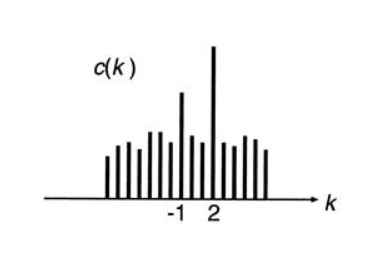
\includegraphics{mafft_correlation_plot}
\caption{Plot of the correlation function $c(k)$. \citep[Figure~1A]{mafft}}
\label{fig:mafft1}
\end{figure}

If we plot the function $c(k)$, there will be some peaks corresponding to the homologous regions of the two sequences, if there are any (Figure \ref{fig:mafft1}). However, the FFT
analysis only gives us the positional lag of the regions, not their positions. To find the exact positions, we use a sliding window (of size 30 in the article)
and calculate the degree of local homologies for the 20 highest peaks in the $c(k)$ function. If a segment exceeding a given homology threshold is identified,
we label it as a homologous region.

\begin{figure}[h]
\centering
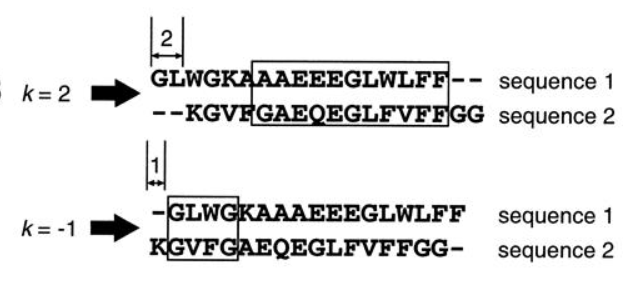
\includegraphics{mafft_sliding_window}
\caption{Finding homologous regions with different positional lags using a sliding window. \citep[Figure~1B]{mafft}}
\label{fig:mafft2}
\end{figure}

After finding homologous segments between two sequences, their alignment is obtained by constructing a homology matrix $S \in R^{n*n}$, where $n$ is the number of homologous
segments. The cell $S_{ij}$ is assigned a value depending on whether the $i$-th homologous segments of the first sequence corresponds to the $j$-th homologous segment
of the second sequence. If so, the cell gets a value corresponding to the score of this segment; otherwise it has a value of 0. The optimal arrangment of homologous segments
is then obtained using dynamic programming.

\begin{figure}[h]
\centering
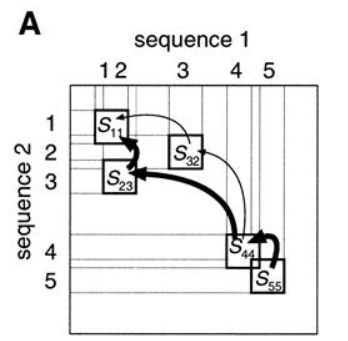
\includegraphics{mafft_optimal_path}
\caption{Dynamic programming applied on segment arrangement. \citep[Figure~2A]{mafft}}
\label{fig:mafft3}
\end{figure}

Having arranged homologous segments, the algorithm then computes pairwise alignments for each pair of sequences. As in T-Coffee, it uses the alignments to create
the primary and extended libraries, which are in turn used to estimate the guide tree and the final alignment. If MAFFT is configured to perform the progressive 
method, this alignment is the final one. Otherwise, if iterative refinement is allowed, MAFFT uses the weights from the library to adjust the alignment to get a more
optimal one. However, iterative refinement is very slow from a relatively low number of sequences, therefore it is not suitable for a large dataset.

\section{Sequence alignment for chant melodies}
\label{section:chant_alignment}

% unlike bioinformatics data, we are working with two sequences - melody and text
% textual boundaries are important as well!
% textual boundaries are important for segmentation of melodies - reference CantusCorpus article

As we have discussed before, melodies of Gregorian chant are in many ways similar to biological sequences. The alphabet is different (instead of 20 amino acids
in proteins or 4 nucleotide bases in DNA we have around 40 different characters used in melody representation) and the chants are usually shorter in length.
The evolution of both biological and melodic sequences is guided by environmental factors such as migration to other places. Some segments tend to undergo a lot
of modifications, while other remain relatively unchanged. Studying the alignment of chant melodies can reveal a lot of information about their relationship.

% merge the following three paragraphs into one
% mention why intervals are important - transposition etc
In the following sections, we describe three approaches to melody alignment used in our application: the naive text-based alignment, .

The first one is a naive approach. It merely aligns all chants to have the same number of words and each word to have the same number of syllables, filling the extra
positions with gaps, if needed.

The other two approaches use MAFFT to perform a proper sequence alignment. They differ in what we are aligning. One of them aligns notes and other symbols as they are;
each representing a certain pitch. The other one is more sophisticated: it does not use the absolute value of the pitches, but rather the intervals between the notes.
This way, we can see segments that have merely been shifted by a certain interval.

\subsection{Word-based alignment}

% baseline - change to basic tool
The word-based approach serves as a basic tool to show the relationship between the text setting and melody.
% something like "the algorithm puts the individual syllables in a row"
% this algorithm is meant primarily for comparing melodies of the same / similar text, such as a chant that belongs to the same liturgial position
The algorithm simply extends all sequences to have the number of words equal to the maximum out of all
sequences, and each word at a position $i$ to have the number of syllables equal to the maximum out of all words at that position. The syllables are then filled
with characters until there are any to use and the remaining ones are left empty.\newline

\begin{algorithm}[H]
\SetKwInOut{Input}{input}\SetKwInOut{Output}{output}
% more formalized data structures text : V_1, ... V_k , words : S_1, S_k
% for each pair (melody, text) there is a function that says which notes start at which position
    \Input{volpiano-encoded melodies $V_1, ..., V_k$; $V_i$ is composed of words $W_{i1}, ..., W_{il}$; $W_{ij}$ is composed of syllables $S_{ij1}, ..., S_{ijm}$;
            the texts corresponding to the melodies}
    \Output{aligned melodies combined with their texts}
    \BlankLine
    $num\_words \longleftarrow max(length(sequence))$ for all sequences\;
    initialize $n$ empty lists of length $num\_words$\;
    \For{word at index i}{
        $num\_syllables \longleftarrow max(length(word))$ for all words at position $i$\;
        set the $i$-th position of each list to be of length $num\_syllables$\;
        \For{syllable at index j}{
            $num\_characters \longleftarrow max(length(syllable))$ for all syllables at position $j$ of words at position $i$\;
            set the $j$-th position of the $i$-th sublist of each sequence to be of length $num\_characters$\;
        }
    }
    \For{each melody}{
        \For{i-th word of melody}{
            \For{j-th syllable of word}{
                fill the $j$-th position of the $i$-th sublist of the list corresponding to the melody with the characters corresponding to the current syllable\;
            }
        }
        % set syllable position in melody according to original placement
        combine the text with the melody\;
    }
    return aligned melodies combined with their texts\;
    \caption{Naive approach to alignment}
    \label{algo:align_naive}
\end{algorithm}

\begin{figure}[h]
\centering
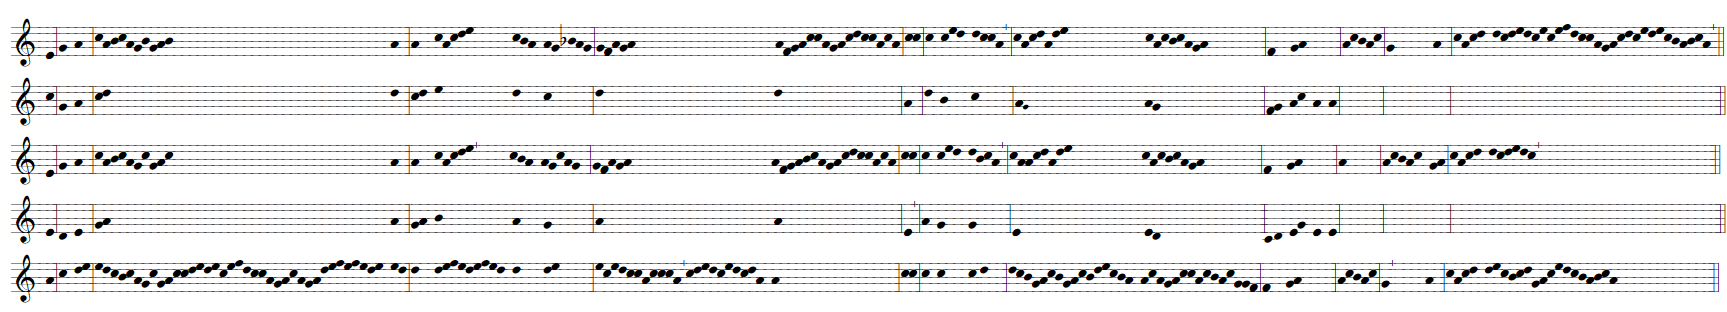
\includegraphics[scale=0.4]{alignment_naive}
\caption{Chants of different genres aligned using the naive approach. The vertical lines represent word boundaries.}
\label{fig:align_naive}
\end{figure}

\subsection{Multiple alignment using absolute pitches}

For this task, we are using the MAFFT software\footnote{\url{https://mafft.cbrc.jp/alignment/software/}}.
MAFFT primarily works for sequences of amino acids and nucleotide bases, but it also has a limited support for non-biological sequences.

%the below into a new subsection

\subsubsection{Melody preprocessing}
\label{section:vol_preprocess}

As the software uses the character \verb|-| for marking gaps,
it requires that the input sequences do not contain any, or they will be removed. Since melodies encoded as Volpiano use the character to mark ends of words
and ends of syllables, we need to perform some preprocessing. Namely, we replace all contiguous sequences \verb|---| with the end-of-word marking symbol \verb|~|
and all contiguous sequences \verb|--| with the end-of-syllable marker \verb=|=. All remaining \verb|-|s are removed, if there are any.

The sequences are then passed to MAFFT with the option \verb|--text|, which indicates that the sequences are not biological. Additionally, we also pass the option
\verb|--reorder|, which returns the aligned sequences in order of similarity. We made this choice so as to facilitate the identification of related melodies.

After MAFFT performs the alignment, we retrieve the sequences and attempt to combine them with their text.
We do this by splitting both the text and the melody into syllables and mapping them onto each other (Algorithm \ref{algo:volpiano_text_combine}). 
However, this might not be possible. Due to errors in the original encoded melody (i.e. a missing or an extra \verb|-|),
we may have altered the structure of the chant in preprocessing. In case of such event, we remove the affected sequence from consideration and align the remaining
sequences again.\newline

\begin{algorithm}[H]
\SetKwInOut{Input}{input}\SetKwInOut{Output}{output}
    \Input{\emph{volpiano}: melody divided into words and those into syllables, and \emph{text}: lyric divided analogically}
    \Output{\emph{volpiano} and \emph{text} aligned}
    \BlankLine
    set \emph{aligned\_text\_and\_melody} to be an empty list\;
    \For{word at index i}{
        open new word in \emph{aligned\_text\_and\_melody}\;
        \uIf{i-th word of text has more syllables than i-th word of melody}{
            merge the extra syllables into the last one\;
        }
        \uElseIf{i-th word of text has fewer syllables than i-th word of melody}{
            extend the i-th word of text by empty syllables to match the volpiano word
        }
        \For{syllable at index j of i-th word}{
            combine text and melody of the j-th syllable of the i-th word and add it to the current word\;
        }
        close current word\;
    }
    return \emph{aligned\_text\_and\_melody}\;
    \caption{Aligning melody and lyric}
    \label{algo:volpiano_text_combine}
\end{algorithm}

Once all sequences are successfully aligned without errors in text and melody combination, we can display them to the user. In the application, we use the Volpiano font,
so as to maintain consistency. However, the sequences shown are not properly encoded following Volpiano protocols. First of all, we choose different representations of end of a word
(here we use a bar line) and end of a syllable (a single space) so that the number of characters in each sequence remains equal and the alignment is visible. Second of all,
after the alignment, MAFFT will have inserted \verb|-|s to represent gaps. In proper Volpiano, these characters represent gaps between words, syllables, and neumes. However,
here they just mean empty space.\newline

\begin{algorithm}[H]
\SetKwInOut{Input}{input}\SetKwInOut{Output}{output}
    \Input{a set of volpiano-encoded melodies with their respective lyrics}
    \Output{aligned melodies combined with their lyrics}
    \BlankLine
    preprocess all melodies to a MAFFT-friendly format\;
    \While{melodies have not been aligned without error}{
        run MAFFT on all melodies\;
        \For{aligned melody}{
            combine melody with its text\;
            \If{melody and text cannot be combined}{
                remove melody from list\;
                remember to run the while loop again\;
            } 
        }
    }
    return list of aligned melodies combined with their texts\;
    \caption{Multiple alignment using absolute pitches}
    \label{algo:align_pitch}
\end{algorithm}

\begin{figure}[h]
\centering
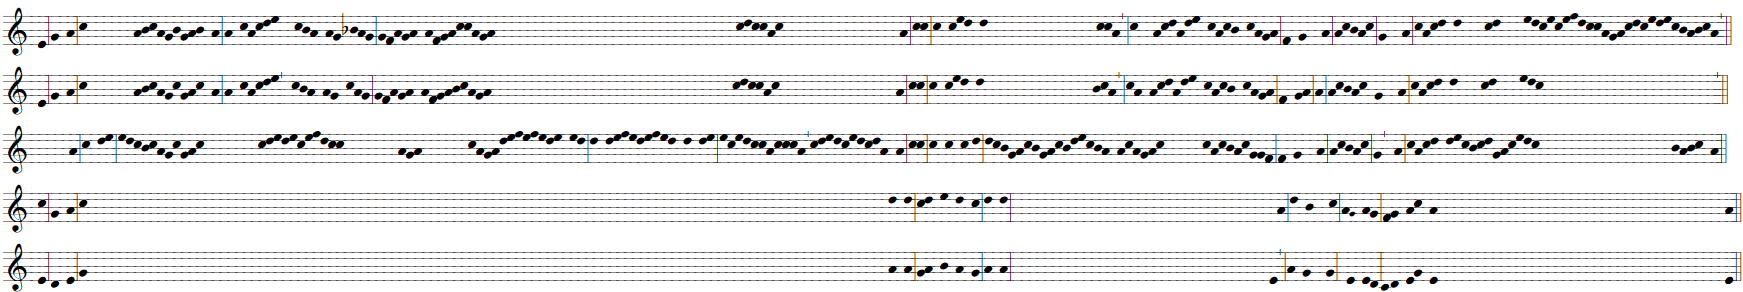
\includegraphics[scale=0.4]{alignment_pitches}
% write that the tildes and pipes from MAFFT are replaced with - and spaces
\caption{Chants aligned using MAFFT on absolute pitches.}
\label{fig:align_pitches}
\end{figure}

\subsection{Multiple alignment using intervals}

The general outline of the algorithm is the same as Algorithm \ref{algo:align_pitch}. However, as we are not aligning absolute pitches, but rather intervals,
we need to compute these intervals.

There are 18 possible pitches, which means 37 possible intervals (17 positive, 17 negative, and one without the change of pitch). We will represent the no-change interval
with the character \verb|a|, the positive intervals with the lowercase characters \verb|b-t| and the negative intervals with the uppercase characters \verb|B-T|. The characters
\verb|i| and \verb|I| are not used for reasons explained later.

The interval representation is constructed from a Volpiano-encoded melody by replacing the note symbols with the appropriate interval symbol. The $i$-th note will be
replaced with the symbol representing the interval $(i-1, i)$. As the first note has no predecessor, it is left as it is. The non-note symbols also remain unchanged.\newline

\begin{algorithm}[H]
\SetKwInOut{Input}{input}\SetKwInOut{Output}{output}
    \Input{volpiano-encoded melody}
    \Output{interval representation of the input melody}
    \BlankLine
    $interval\_representation \longleftarrow ""$\;
    \For{character c in volpiano}{
        \uIf{c is a non-note character}{
            append c to \emph{interval\_representation}\;
        }
        \uElseIf{c is a note-representing character and it is the first such one}{
            append c to \emph{interval\_representation}\;
            $last\_seen\_note \longleftarrow c$\;
        }
        \uElse{
            $interval \longleftarrow (last\_seen\_note, c)$\;
            $i \longleftarrow symbol \: for \: interval$\;
            append i to \emph{interval\_representation}\;
            $last\_seen\_note \longleftarrow c$\;
        }
    }
    return \emph{interval\_representation}\;
    \caption{Converting volpiano-encoded melody into interval representation}
    \label{algo:convert_to_interval}
\end{algorithm}

We use the interval representations as inputs to MAFFT. That means that what MAFFT returns are the aligned sequences of intervals. To display them to the user
properly, we need to decode the sequences.\newline

\begin{algorithm}[H]
\SetKwInOut{Input}{input}\SetKwInOut{Output}{output}
    \Output{interval representation of a melody}
    \Input{volpiano-encoded equivalent of the input melody}
    \BlankLine
    $volpiano \longleftarrow ""$\;
    \For{character c in interval representation}{
        \uIf{c is a non-interval character}{
            append c to \emph{volpiano}\;
        }
        \uElseIf{c is a note-representing character and it is the first such one}{
            append c to \emph{volpiano}\;
            $last\_seen\_note \longleftarrow c$\;
        }
        \uElseIf{c is an interval-representing character and we have already seen the first note}{
            $note \longleftarrow last\_seen\_note +$ interval represented by $i$\;
            append note to \emph{volpiano}\;
            $last\_seen\_note \longleftarrow note$\;
        }
    }
    return \emph{volpiano}\;
    \caption{Converting interval representation back to volpiano}
    \label{algo:decode_interval}
\end{algorithm}

% reformulate
% the reason why i and I do not represent an interval is that they 

% to introduction - chant uses diatonic scale with the 7th having two versions (with becko) - ignoring b is legitimate
The reason why we are not using \verb|i| and \verb|I| as symbols for an interval is that as we are looking at whether a character is a note or an interval or neither, 
if they represented an interval, we would choose the appropriate branch in Algorithm \ref{algo:decode_interval}. However, marking an interval is not the only way how
the character could have got there: \verb|i| and \verb|I| represent non-note elements in the Volpiano protocol. Therefore, we could mistakenly shift the melody by an interval,
as there is no way of knowing which case it is.

The complete Algorithm \ref{algo:align_intervals}, similar to Algorithm \ref{algo:align_pitch}:\newline

\begin{algorithm}[H]
\SetKwInOut{Input}{input}\SetKwInOut{Output}{output}
    \Input{a set of volpiano-encoded melodies with their respective lyrics}
    \Output{aligned melodies combined with their lyrics}
    \BlankLine
    convert all melodies to interval representations\;
    preprocess all interval representations to a MAFFT-friendly format\;
    \While{melodies have not been aligned without error}{
        run MAFFT on all interval representations\;
        \For{aligned interval representation}{
            convert interval representation to volpiano-encoded melody\;
            combine melody with its text\;
            \If{melody and text cannot be combined}{
                remove melody from list\;
                remember to run the while loop again\;
            } 
        }
    }
    return list of aligned melodies combined with their texts\;
    \caption{Multiple alignment using intervals}
    \label{algo:align_intervals}
\end{algorithm}

\begin{figure}[h]
\centering
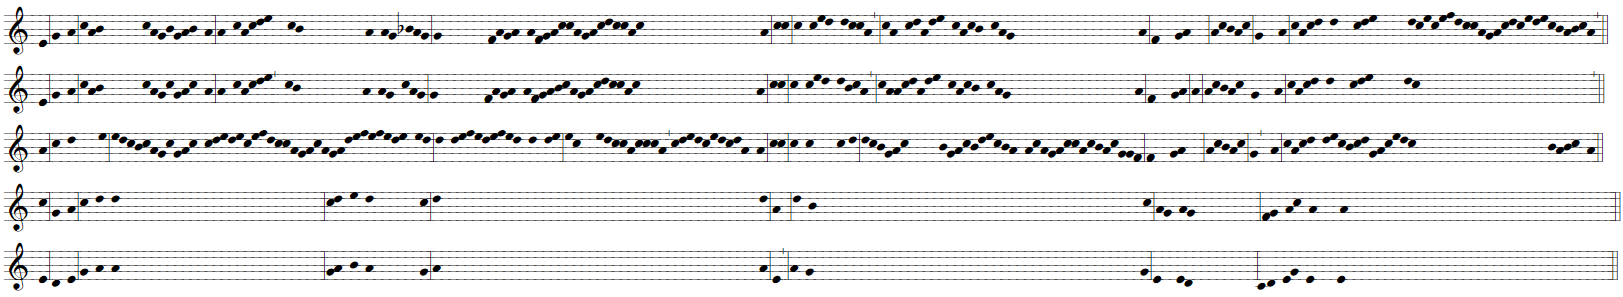
\includegraphics[scale=0.4]{alignment_intervals}
\caption{Chants aligned using MAFFT on intervals.}
\label{fig:align_intervals}
\end{figure}

\section{Conservation profile}

% we can borrow other bioinformatics characteristics after having computed an alignment

By obtaining an alignment of a set of chants, we can obtain an interesting characteristic which is called the \emph{conservation profile}. We define the conservation value
of an element $a$ at position $i$ as 

\[
    con_i(a) = \frac{\sum_{C: C_i = a} 1}{\sum_C 1}
\]
where $C$ denotes a chant and $C_i$ the element at position $i$ in the aligned chant $C$. In other words, the conservation value gives the ratio of elements $a$
at position $i$ out of all chants.

% conservation profile is a vector with the average of conservation values
% we visualize something different

Conservation profile of aligned sequences depends on what approach we choose. Consider the last two chants shown in Figure \ref{fig:align_intervals}. Each note
is different, however, a person well-versed in musical theory immediately notices that they are only shifted by 5 semitones (except for the first note). If we consider only
the intervals, they are almost the same melodies. However, if we consider the absolute pitches, they are totally different. Figure \ref{fig:cons_pitch}
and Figure \ref{fig:cons_intervals} demonstrate these differences by displaying the chants' conservation profile.

\begin{figure}[h]
\centering
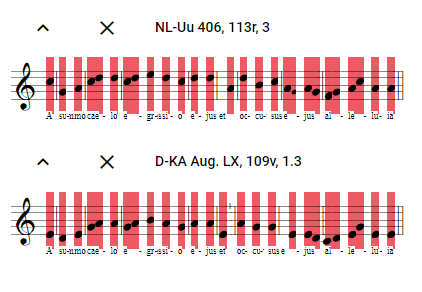
\includegraphics{alignment_antiphons_pitches}
\caption{Conservation profile on chants aligned by pitch.}
\label{fig:cons_pitch}
\end{figure}

\begin{figure}[h]
\centering
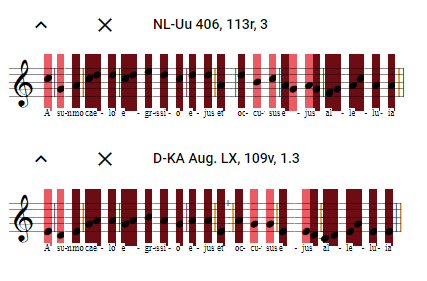
\includegraphics{alignment_antiphons_intervals}
\caption{Conservation profile on chants aligned by intervals.}
\label{fig:cons_intervals}
\end{figure}

% the natural next step would be to compute the phylogenetic tree which we did not do

% write why we do three different alignments
% kontrafakta for 3.2
